% !TEX root = template.tex

\section{Results}
\label{sec:results}

\begin{table*}[t]
	\begin{center}
		\begin{tabular}{ p{7cm}p{2cm}p{2cm}p{2cm}p{2cm} } 
			\hline
			Method & Accuracy & Precision & Recall & F1-Score \\ 
			\hline
			CNN + No centering & 77,0 & 78,0 & 75,8 & 76,8 \\ 
			CNN + No centering + Manual F. & 75,6 & 76,8 & 73,9 & 75,3 \\
			CNN + Centering + Manual F. & 86,2 & 86,9 & 70,2 & 77,6 \\ 
			\textbf{CNN + Centering + Encoder F.} & \textbf{89,2} & \textbf{88,9} &  \textbf{86,1} & \textbf{86,1} \\ 
			\hline
		\end{tabular}
	\caption{\label{tab:model-performance} UCI classification results with different featueres CNN augumentation and data preprocessing, using 196 conv. filters and 64 dense neurons}
	\end{center}
\end{table*}

\begin{table}
	\begin{center}
		\begin{tabular}{ p{1.8cm}p{1.7cm}p{1.7cm}p{1.7cm} } 
			\hline
			CNN Filters & Dense Neurons & Accuracy & F1-Score \\ 
			\hline
			196 & 1024 & 84,6 & 75,3 \\
			196 & 512 & 86,1 & 75,7 \\ 
			\textbf{196} & \textbf{64} & \textbf{88,9} & \textbf{81,6} \\ 
			96 & 1024 & 82,8 & 69,9 \\
			96 & 512 & 84,4 & 73,7 \\ 
			96 & 64 & 89,0 & 73,0 \\  
			48 & 1024 & 80,0 & 79,4 \\
			48 & 512 & 83.7 & 74.9 \\ 
			48 & 64 & 84,0 & 72,3 \\
			\hline
		\end{tabular}
	\caption{\label{tab:model-selection} UCI classification results with data centering and manual features augmented CNN}
	\end{center}
\end{table}

\begin{figure}[h]
  \centering
  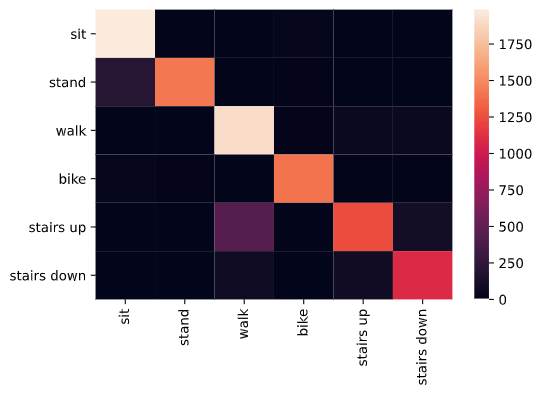
\includegraphics[width=0.5\textwidth]{images/confusion_matrix.png}
  \caption{CNN confusion matrix}
  \label{fig:cnn-confusion-matrix}
\end{figure}

Io direi che in questa parte partiamo con il dataset eterogeneo, facendo vedere come si comporta anche con le posizione sit e stand, e dopodichè passando ai risultati ottenuti con il rotational indipendent far vedere quello che abbiamo ottenuto nel dataset nostro, dove le attivita' sit e stand sono state compressate in no\_activity!

\subsection{Original settings}

Parlare dei risultati ottenuti da luca con un semplice autoencoder sia K-NN classifier che con FFNN alla fine. Un concetto alla volta!

Passare alla mia archittetura e spiegare come sono stati scelti i paramentri, poi far vedere che togliende le basic feature il modello decrementa la sua accuracy, e aggiungendo invece quelle de''autoencode il modello migliora. 

Calcolare anche la F1 score e prbabilmente abbiamo migliorato di molto il modello proposto in \cite{blunck2013heterogeneity}

\subsection{Advance settings}
Passare al nostro dataset e far vedere l'importanza del rotational invariant!!! Che migliora sensibilmente le performance ovviamente dato che la rete è allenata in posizione fisse.

RIPORTARE TUTTE LE METRICHE, anche confusion matrix e argomentarle
